\section{NuMI $\nu_{\lowercase{e}}$~+~$\bar{\nu}_{\lowercase{e}}$ Selection}\label{numi_nue_selection}

This chapter describes a set of cuts chosen to distinguish electron neutrino interactions from various backgrounds coming from cosmic ray and beam-induced interactions. This selection is inclusive, meaning all permutations of an electron neutrino or electron antineutrino charged current (CC) interaction should be part of the signal definition. The only required reconstructed feature is the presence of a shower. Because MicroBooNE is not able to differentiate electrons from positrons, and therefore $\nu_e$ versus $\bar{\nu}_e$, the resulting selection will contain both particles. This also means that the cross section calculated in Chapter \ref{chapter_cross_section} includes both $\nu_e$ and $\bar{\nu}_e$ events. For simplicity and because the flux is dominated by electron neutrinos, $\nu_e$ is used to refer to both $\nu_e$ and $\bar{\nu}_e$ events in this chapter. 

%%%%%%%%%%%%%%%
\subsection{Selection Overview}

A variety of selection cuts are applied to select the $\nu_e$ CC interactions from among the much larger backgrounds. Some selection cuts are generic and target all or most backgrounds, while some are used to reduce specific backgrounds. A high-level diagram of the selection cut groups is shown in Figure \ref{cut_flow_diagram}, where each group contains a number of specific cuts. The selection cut groups are briefly explained below and then individually explained in the following sections.

\begin{figure}[htbp]
\center
\includegraphics[width=0.6\textwidth]{plots_main/cut_flow_diagram_2.png}
\caption{Overview of selection cut categories applied in this analysis. Cuts in group \textbf{(1)} are pre-cuts used to construct the signal definition. Cut \textbf{(2)} involves matching between optical and TPC information. TPC Object quality cuts \textbf{(3)} try to remove showers and tracks far from the neutrino vertex. Hit thresholds \textbf{(4)} aim to target cosmic ray backgrounds and again improve the quality of reconstructed showers. Removal of photon-like and mis-reconstructed showers is the goal of the cuts in group \textbf{(5)}. Lastly, a combination of small improvements in group \textbf{(6)} finalise the selection.}
\label{cut_flow_diagram}
\end{figure}

\FloatBarrier
\begin{itemize}

    %\item \textbf{Reconstruction Pass 2:} This is the final level of reconstruction achieved by Pandora. At this stage, the neutrino interaction is reconstructed, but makes no requirement regarding its topology.
    
    %\item\textbf{Flash ``In Time'':} A reconstructed optical event (a flash), is within the timing window during which neutrinos are expected to arrive at the detector. This time window is delivered from the accelerator division at Fermilab, while the flash is reconstructed using MicroBooNE's PMTs.
    
    %\item \textbf{Flash Photoelectron Count:} A threshold placed to ensure the flash is above a noise level of 50 PE.
    
    \item \textbf{(1) Simple Selection Pre-Cuts:} The reconstructed neutrino interaction must be identified by \textit{PANDORA} to be $\nu_e$-like. This means that a shower was reconstructed from the interaction and has a greater number of hits than any reconstructed tracks. The interaction must also contain an optical flash correlated with the NuMI accelerator signal and the flash size must be larger than 50 PE. Lastly, the reconstructed neutrino vertex must be inside the fiducial volume.
    
    %\item \textbf{Reco. Vertex in Fid. Vol.:} The reconstructed neutrino vertex is within the fiducial volume, which is taken to be 20 cm from all sides of the TPC.
    
    \item \textbf{(2) Flash Matching:} The relationship between the reconstructed optical information and the reconstructed TPC information is used to make this cut. The distance between the largest flash and the reconstructed neutrino vertex is calculated and used to reject cosmic backgrounds. 
        
    %\item \textbf{Shower to $\nu$ Vertex:} For event quality, a maximum distance is allowed between the reconstructed leading shower vertex and the reconstructed neutrino vertex. Currently this distance is 4 cm.
    
    %\item \textbf{Track to $\nu$ Vertex:} Also for event quality, a maximum distance is allowed between the reconstructed track vertex and the reconstructed neutrino vertex. Currently this distance is 4 cm.
    
    \item \textbf{(3) Reconstructed Vertex Quality:} The distance between the reconstructed neutrino vertex and corresponding tracks or showers cannot exceed 4 cm. If the leading shower or any tracks are further than 4 cm away, the TPC Object is rejected.
    
    %\item \textbf{Hit Threshold:} A minimum threshold is set for the leading shower's wire plane activity. The threshold is set to 200 hits and is summed across all three planes.
    
    \item \textbf{(4) Shower Hit Threshold:} A minimum threshold is set for the leading shower wire plane activity. This takes two forms, first a minimum of 200 hits across all three wire planes is required. Second, the leading shower must have at least 80 hits on the collection plane (Y-Plane).
    
    \item \textbf{(5) Electron-like Showers:} Cuts on the leading shower opening angle and dE/dx remove both mis-reconstructed tracks and photon-like showers.
    
    %\item \textbf{$>$1 Shower to $\nu$ Distance:} Certain reconstructed events have spurious secondary showers distanced far from the reconstructed neutrino vertex. Events which have more than one shower are subject to the requirement that the secondary reconstructed showers be within 22 cm of the reconstructed neutrino vertex.
    
    %\item \textbf{Leading Shower Hits Per Length:} To try and remove tracks which have been reconstructed as showers, the leading shower is required to have at least 3 hits per 1 cm in length. The hits are summed across all wire planes and the length is calculated based on the projection along the primary shower axis.
    
    %\item \textbf{Track Shower Ratio:} Again with the purpose of removing tracks which have been reconstructed as showers, the ratio of the leading shower length to longest track length is required to be at least 1:1.
    
    \item \textbf{(6) Final Tuning:} A number of small cuts aimed at removing tracks which were reconstructed as showers, originating primarily from cosmic interactions. These involve rejecting TPC Objects based on properties such as the number of hits per unit length, the ratio of the shower to track lengths and track containment.

\end{itemize}

%%%%%%%
\subsection{Simple Pre-Cuts}

\subsubsection{Shower Finding}

When \textit{PANDORA} reconstructs particles they are classified as either tracks or showers. The first selection cut requires at-least one reconstructed shower associated to the TPC Object. This shower is also required to be the object with the most charge collected of all associated reconstructed objects. This means that the TPC Object is identified by \textit{PANDORA} as a reconstructed $\nu_e$ interaction. The shower with the most hits is defined as the ``leading shower'' and is commonly referred to in many selection cuts. %In the case that two showers are associated to the TPC Object, the shower with the most hits is classified as the leading shower.

%%%%%%%%%%%%%%%%%%%%%%%%%%%%%%%%%%%%%%%%%%%%%%%%%%%%%%%
\subsubsection{Scintillation-Based Timing Cut} \label{section_optical_cuts}

Scintillation light is fast (ns) compared to charge collection (ms), and is therefore better suited for determining the interaction time of the particle. The time during which the NuMI beam spill occurs and when neutrinos are expected at MicroBooNE is known from the timing provided by the Fermilab Accelerator Division. This selection cut is constructed by checking if the flash produced by the interaction is coincident with the NuMI beam spill. 

The distribution of the reconstructed flash timepre_hit_cut_total_hits_leading_shower_data is shown in Figure \ref{flash_time_data_everything} for data versus the stacked prediction of NuMI EXT + Dirt Monte Carlo + NuMI Monte Carlo, where 5.5 to 16.0 $\mu$s corresponds to the NuMI beam spill. Thus, flashes reconstructed outside the window of 5.5 to 16.0 $\mu$s are rejected. Large peaks in the flashes around 0 and 1 $\mu$s are artefacts of the software trigger and do not affect the performance of the selection cut. The rise in flashes primarily from the NuMI EXT and On-Beam datasets between 2 and 4.5 $\mu$s is pollution from other trigger streams (flashes during BNB EXT trigger for example). Flashes between 17 and 20 $\mu$s are generated mainly by late-light scintillation. Disagreement between On-Beam data and prediction around 12 to 15 $\mu$s are a result of the slip-stacking configurations (Section \ref{section_slip_stacking}). This disagreement is discussed further in Section \ref{section_systematics_slip_stacking} and should have no impact on selection performance.

\begin{figure}[htbp]
\center
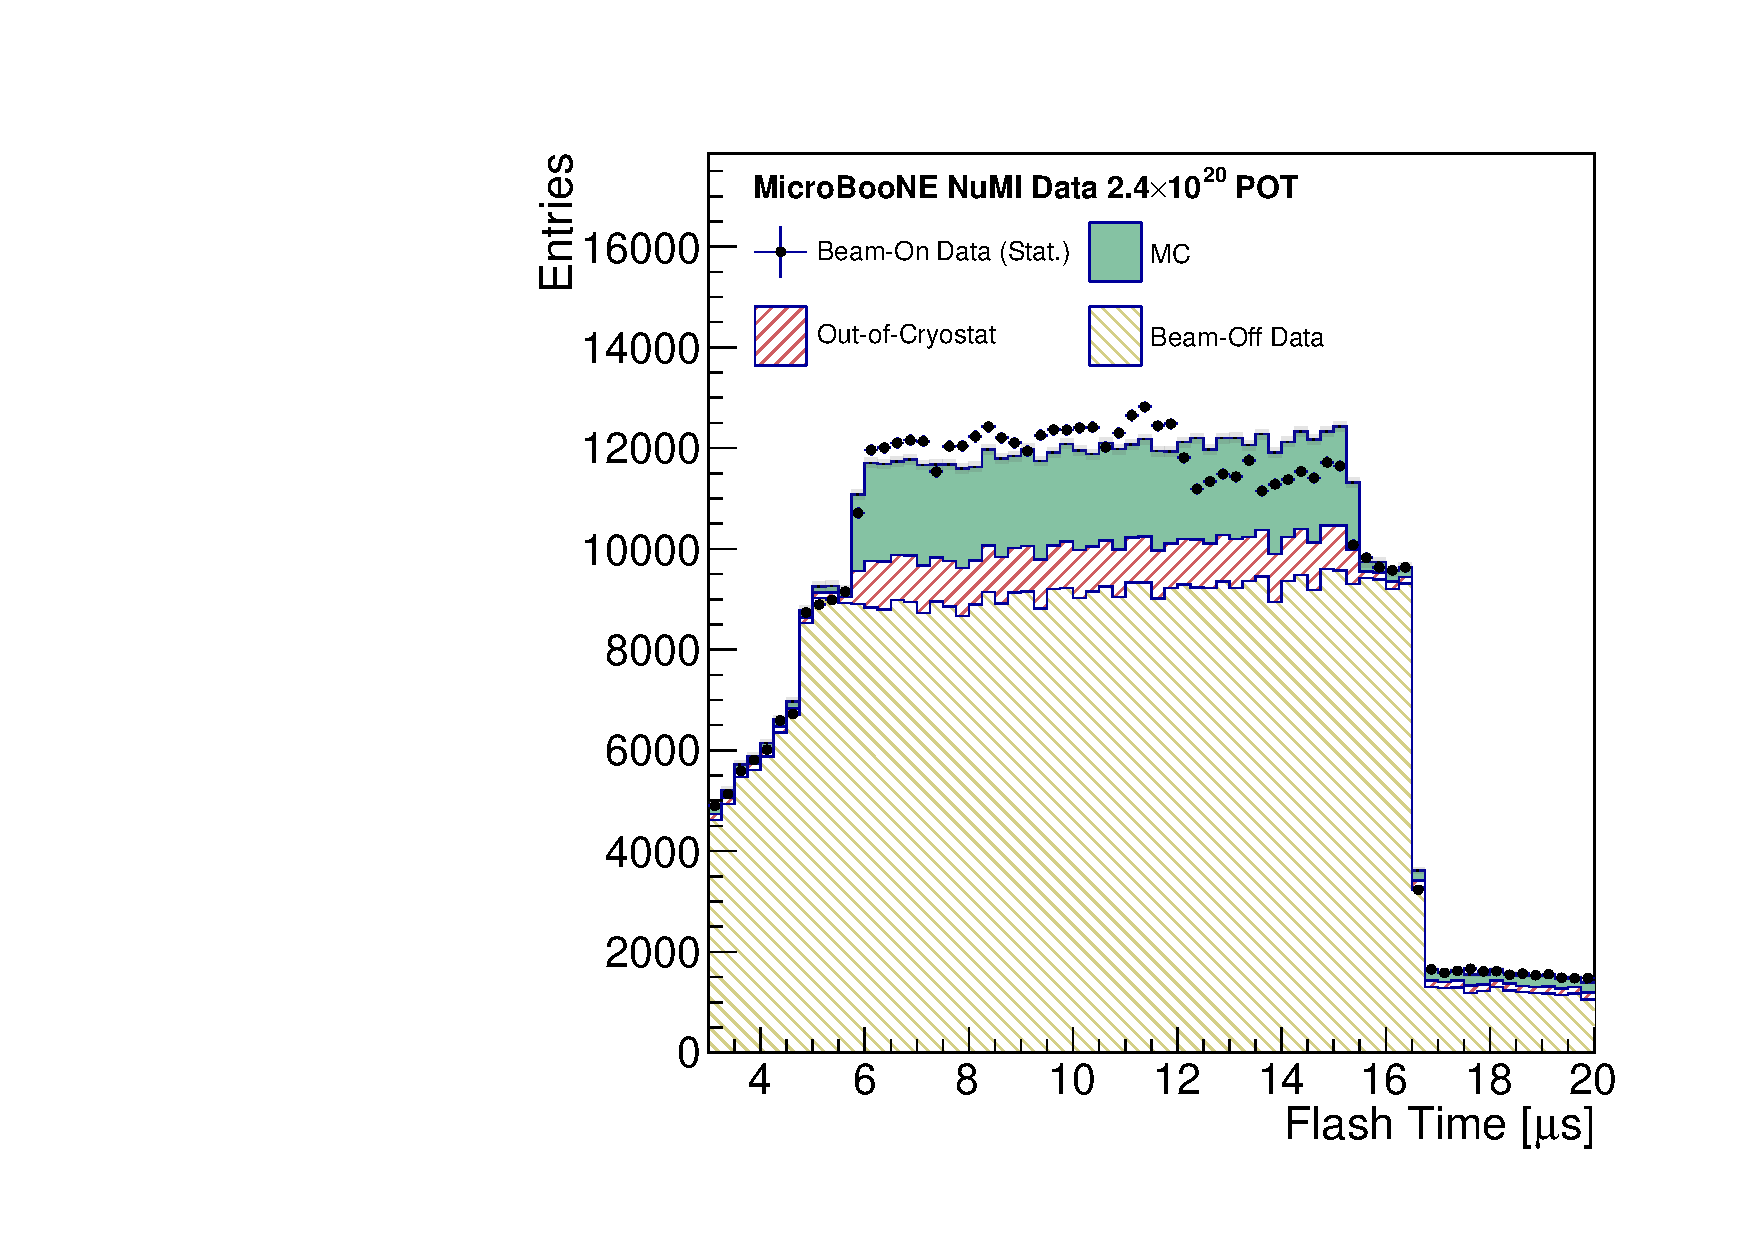
\includegraphics[width=0.6\textwidth]{plots/flash_time_data_everything.pdf}
\caption{On-Beam data (points) compared to prediction (NuMI EXT + Dirt Monte Carlo + Beam Monte Carlo) for the reconstructed flash time before selection cuts are applied. The NuMI beamspill occurs between 5.5 and 16.0 $\mu$s, where the greatest number of flashes are observed. Due to differences in the trigger board, there is a small (22 tick) offset between the On-Beam and Off-Beam timing. Given the sampling rate of 64 MHz, the offset is calculated as: $22 / 64$ MHz $= +343$ ns. This creates the observed difference of the earliest entries for the different types of data.}
\label{flash_time_data_everything}
\end{figure}

\subsubsection{Flash Amplitude}

The amplitude of the flash, or how many photoelectrons (PE) are collected, is somewhat correlated to the energy deposited in the detector. Due to non-uniformity in the light yield of MicroBooNE, calculating the deposited energy of the flash independent of its position is difficult. Nonetheless, a large fraction of cosmic rays which interact in the detector deposit less average energy than even the lower energy neutrinos. A PE threshold on the lower-bound can be set to exclude these background events. 50 PE was found to be sufficiently low such that signal events have 99\% efficiency, but high enough to remove a significant number of low energy cosmic rays.

\FloatBarrier
%%%%%%%%%%%%%%%%%%%%%%%%%%%%%%%%%%%%%%%%%%%%%%%%%%%%%%%%%%
\subsubsection{Fiducial Volume}\label{section_fv_cut}

The MicroBooNE cryostat extends beyond the instrumented portion of the TPC. Particles which interact outside of the instrumented region can enter into the TPC, resulting in interactions that are difficult to resolve. A fiducial volume cut is applied around the sides of the TPC to ensure that interactions can be fully resolved, minimising edge-effects and accounting for about 1.5 radiation lengths.

Figure \ref{pre_cuts_leading_pfp_xyz_data} shows the distribution of reconstructed neutrino vertices before any cuts are applied. The shapes of these distributions arise through various detector effects. In the $X$ direction, the number of vertices increases towards the cathode. This is a result of the Space-Charge Effect, where the electric-field distortions affect the reconstructed vertex position. The $Y$ distribution sees an increase in vertices near the edges of the TPC due to cosmic rays. These cosmic rays are often reconstructed as either downward-going (placing the vertex at the top of the TPC), or incorrectly reconstructed as going upwards (placing the vertex at the bottom of the TPC). The shape of the $Z$ distribution comes from slight variations in electronics performance across the TPC and how this is modelled in data versus Monte Carlo. 

\begin{figure}[htbp]
\center
\includegraphics[width=0.48\textwidth]{plots/post_cuts_leading_pfp_x_data.pdf}
\includegraphics[width=0.48\textwidth]{plots_main/post_cuts_leading_pfp_y_data.pdf}
\includegraphics[width=0.48\textwidth]{plots/post_cuts_leading_pfp_z_data.pdf}
\caption{Comparison of data (points) to the stacked prediction (Monte Carlo + NuMI EXT). (Left) Reconstructed $X$ position of all TPC Objects with at least one shower. The enhancement in the $X$ direction is due to space charge effects. (Right) Reconstructed $Y$ position of all TPC Objects with at least one shower. Bins at high $Y$ are near the top of the detector, where the majority of cosmic rays interact. (Bottom) Reconstructed $Z$ position of all TPC Objects with at least one shower. Dips in number of vertices correspond to sections of the TPC where there are unresponsive wires.}\label{pre_cuts_leading_pfp_xyz_data}
\end{figure}

%%return - chi2 calculation and some values are too small! --> looks like it's basically only the X plot, maybe just a bug
%%return - Costas makes point that cosmic and InTime shape don't agree --> is it just the plotting or true? If they're actually different, need to assign another uncertainty??? (there is one already, but should be bigger?) --> they largely agree actually

The vertices can also be examined in 2D by looking at the TPC from a side-on view. The $YZ$ plane is shown in Figure \ref{pre_cuts_leading_pfp_zy_data}, where the majority of signal TPC Objects are reconstructed at-least 10 cm from the edges of the TPC. This is compared to the cosmic rays from the NuMI EXT trigger stream, which are concentrated around the top and, to a lesser extent, bottom of the detector.

\begin{figure}[htbp]
\center
\includegraphics[width=0.48\textwidth]{plots_main/pfp_zy_vtx_nue_cc.pdf}
\includegraphics[width=0.48\textwidth]{plots_main/pfp_zy_vtx_ext.pdf}
\includegraphics[width=0.48\textwidth]{plots_main/pfp_zy_vtx_all_norm_z.pdf}
\includegraphics[width=0.48\textwidth]{plots_main/pfp_zy_vtx_data_norm_z.pdf}
\caption{(Top-Left) $YZ$ distribution of reconstructed TPC Object vertices for true signal TPC Objects. Vertices are rather evenly distributed throughout the detector volume. (Top-Right) $YZ$ distribution of reconstructed TPC Object vertices for Off-Beam events. Interactions are evenly located throughout the detector, apart from heavy pile-up near the top, and to a lesser extent, the bottom of the TPC. (Bottom-Left) All Monte Carlo (signal + background) and Off-Beam TPC Objects plotted together as a distribution of the reconstructed vertex in $YZ$. This is compared to the Bottom-Right plot which shows the TPC Object vertices for all On-Beam data. If the normalisation has been performed correctly, the Bottom-Left and Bottom-Right plots are expected to agree.}\label{pre_cuts_leading_pfp_zy_data}
\end{figure}

To obtain both a sample of contained showers in the TPC and remove cosmic rays near the top and bottom of the detector, a fiducial volume cut is applied to the reconstructed vertex. The dimensions of the fiducial volume are shown in Table \ref{fiducial_volume_dimensions}. Any TPC Object with a reconstructed vertex outside of these dimensions is removed.

\begin{table}[htbp]
\begin{center}
\begin{tabular}{l | l | l}
%\hline
\hline
Dimension & Minimum [cm] & Maximum [cm]\\
\hline
 X & 20 & 236.35 \\
 Y & -96.5 & 96.5 \\
 Z & 20 & 1016.8 \\
%\hline
\hline
\end{tabular}
\end{center}
\caption{Dimensions of the MicroBooNE TPC following a fiducial volume requirement removing 20 cm uniformly from all sides of the TPC. TPC Objects with a reconstructed vertex outside the volume are removed.}
\label{fiducial_volume_dimensions}
\end{table}

\FloatBarrier
%%%%%%%%%%%%%%
\subsubsection{Pre-selection Cuts Summary}

The set of simple pre-cuts presented in this section required: a reconstructed TPC Object with a shower as the largest associated particle, a reconstructed flash coincident with the NuMI beam spill, the flash having at-least 50 PE in amplitude and the TPC Object vertex within the defined fiducial volume. These cuts are the starting-point for the selection.

The efficiency of the selection throughout this chapter is calculated using the number of reconstructed $\nu_e$ CC events which pass the selection cuts as the numerator and the number of true $\nu_e$ CC events in the fiducial volume as the denominator. The starting efficiency for the selection becomes $\epsilon = 3899 / 7103 = 54.89\%$. This large initial loss in efficiency is primarily driven by the shower reconstruction performance, where the electron in the $\nu_e$ CC interaction is often reconstructed either as a track or not at all. Recovering these interactions would likely require considerable work to do correctly and could be a clear area for improvement either at reconstruction or selection level.

The other metric used to track the performance of the selection is the purity. Purity is simply defined as the number of selected signal events divided by the total number of selected TPC Objects. The breakdown of the selected TPC Objects according to the classification types defined in Section \ref{section_event_classification} are shown in Table \ref{selection_summary_table_fv}. All values in the table have been normalised to the POT of the On-Beam data. At this stage, the purity is only 0.74\%, with cosmic rays being the largest background by-far. 

\begin{table}[htbp]
\center
\begin{tabular}{l | l l }
Classification & Num. Remaining \\
\hline
$\nu_e$ CC & 507.26 \\
$\nu_e$ CC Mixed & 134.00 \\
$\nu_e$ CC OutFV & 93.15 \\
$\nu_{\mu}$ CC & 1749.84\\
NC & 201.92 \\
NC $\pi^0$ & 843.96 \\
NC Mixed & 227.42 \\
Unmatched & 384.84 \\
Cosmic & 7736.40 \\
InTime & 52838.40 \\
Dirt &4128.52 \\
\hline
\hline
Efficiency & 54.89\%\\
Purity & 0.74\%\\
\hline
On-Beam Data & 70691\\
\hline
\end{tabular}
\caption{Breakdown of remaining TPC Objects by classification type following the pre-selection cuts, normalised to the On-Beam POT.}\label{selection_summary_table_fv}
\end{table}

\FloatBarrier
%%%%%%%%%%%%%%%%%%%%%%%%%%%%%%%%%%%%%%%%%%%%%%%%%%%%%%%%%%
\subsection{Flash Matching}

A powerful method to reject cosmic ray backgrounds is to combine the TPC and light information. This is known as ``flash-matching'', and uses the centre of the largest flash (most PE) in a given event and compares it to the reconstructed \textit{PANDORA} vertices in 2D ($YZ$ plane). This distance can be used to distinguish cosmic rays from beam-induced interactions. The distinguishing power comes from neutrino events producing more light on average than cosmic rays.

%%awkward??%%
The reconstructed flash position in $Z$ is shown in Figure \ref{flash_z_data}. On-Beam data is compared to the stacked prediction and shows agreement to within a few percent in most regions. The shape of the distribution is defined by the layout of the PMTs across the $YZ$ plane of the detector, where the five peaks align with the five groups of PMTs.

Combining the flash position information with the reconstructed TPC Object vertices examined earlier, the 2D distance between these positions can be constructed as:

\begin{equation}
\Delta YZ = \sqrt{(z_{Flash} - z_{TPC})^{2} + (y_{Flash} - y_{TPC})^{2}}~,
\end{equation}

\noindent where $z_{Flash}$ and $y_{Flash}$ are the reconstructed vertex of the largest flash and $z_{TPC}$ and $y_{TPC}$ are the reconstructed TPC Object vertex location. $\Delta YZ$ is then plotted for each TPC Object in Figure \ref{post_cuts_vtx_to_flash_distance_data}, which includes the Y-axis plotted normally and as Log(Y) to make the signal distribution more visible. Around 80 cm, the distribution of signal TPC Objects mostly disappears, leaving primarily Off-Beam and simulated cosmic backgrounds at greater values.

\begin{figure}[htbp]
\center
\includegraphics[width=0.6\textwidth]{plots/flash_z_data.pdf}
\caption{Comparison of data (points) to the stacked prediction (Monte Carlo + NuMI EXT) for the largest flash centre in $Z$ before selection cuts are applied is shown here.}\label{flash_z_data}
\end{figure}

\begin{figure}[htbp]
\center
\includegraphics[width=0.48\textwidth]{plots/post_cuts_vtx_to_flash_distance_data.pdf}
\includegraphics[width=0.48\textwidth]{plots_main/post_cuts_vtx_to_flash_distance_data_logy.pdf}
\caption{Comparison of data (points) to the stacked prediction (Monte Carlo + NuMI EXT) for the 2D distance ($YZ$) between the largest reconstructed flash and all reconstructed neutrino vertices. This case presents the uniform (symmetric) cut, agnostic of the relative flash position along $Z$. Beam-induced TPC Objects are mainly at lower distances, while cosmic-induced (Off-beam and CORSIKA overlay) are primarily at larger distances (greater than 80 cm). The right plot shows the Log(Y) axis.}\label{post_cuts_vtx_to_flash_distance_data}
\end{figure}

\begin{samepage}

The performance of the cut can be improved by using the relative position of the flash w.r.t the TPC Object vertex. This creates two different threshold values: one where the TPC Object vertex $Z$ is greater than the flash $Z$ and vice versa. Figure \ref{post_cuts_vtx_to_flash_distance_upstream_data} shows shifts in the distribution when these two datasets are separated. When the TPC Object $Z$ is greater than the flash $Z$, the distribution of signal interactions has a smaller tail extending to values greater than 60 cm, allowing the selection cut to be tightened. The final cut values are therefore:

\begin{equation}
\begin{split}
z_{TPC} > z_{Flash} \rightarrow \Delta YZ < 80~\textrm{cm}~,\\
z_{TPC} < z_{Flash} \rightarrow \Delta YZ < 60~\textrm{cm}~.
\end{split}
\end{equation}

\end{samepage}

\begin{figure}[htbp]
\center
\includegraphics[width=0.48\textwidth]{plots/post_cuts_vtx_to_flash_distance_upstream_data.pdf}
\includegraphics[width=0.48\textwidth]{plots/post_cuts_vtx_to_flash_distance_downstream_data.pdf}
\caption{Comparison of data (points) to the stacked prediction (Monte Carlo + NuMI EXT) for the 2D distance ($YZ$) between the largest reconstructed flash and all reconstructed neutrino vertices. (Left) Flash is downstream in $Z$ w.r.t the reconstructed neutrino vertex. The signal TPC Objects, along with other beam-induced TPC Objects are clearly enhanced at lower values compared to the cosmic-induced. Cut value is maintained at 80 cm. (Right) Flash is upstream in $Z$ w.r.t the reconstructed neutrino vertex. This case contains a lower signal-background ratio, and a smaller tail for signal TPC Objects, resulting in a tightening of the cut value to 60cm.}\label{post_cuts_vtx_to_flash_distance_upstream_data}
\end{figure}

The final performance of the flash-matching cut is shown in Table \ref{selection_summary_table_flash_to_vtx}, together with the relative reduction in the number of TPC Objects compared to the number remaining from the previous set of cuts. This cut has an overall high-impact, reducing the cosmic ray backgrounds by almost 90\% and increasing the purity to a total of 3.57\%.

\begin{table}[htbp]
\center
\begin{tabular}{l | l l }
Classification & Num. Remaining & Rel. Remaining [\%] \\
\hline
$\nu_e$ CC & 351.14 & 69.22\\
$\nu_e$ CC Mixed & 71.03 & 53.00\\
$\nu_e$ CC OutFV & 30.18 & 32.40\\
$\nu_{\mu}$ CC & 893.66 & 51.10\\
NC & 123.08 & 60.95\\
NC $\pi^0$ & 528.21 & 62.59\\
NC Mixed & 100.83 & 44.34\\
Unmatched & 80.92 & 21.03\\
Cosmic & 613.68 & 7.93\\
InTime & 6642.75 & 12.57\\
Dirt & 403.88 & 9.78\\
\hline
\hline
Efficiency & 38.00\%\\
Purity & 3.57\%\\
\hline
On-Beam Data & 11135\\
\hline
\end{tabular}
\caption{Breakdown of remaining TPC Objects following the flash-matching cut by classification type, normalised to the On-Beam POT. The relative percentages are compared to the values following selection cuts in group \textbf{(1)} (see Figure \ref{cut_flow_diagram}).}\label{selection_summary_table_flash_to_vtx}
\end{table}

\FloatBarrier
%%%%%%%%%%%%%%%%%%%%%%%%%%%%%%%%%%%%%%%%%%%%%%%%%%%%%%%%%%
\subsection{Vertex Reconstruction Quality}

In some cases the reconstruction of the individual Particle Objects and/or the TPC Object can fail. This can be reflected in the track or shower vertex being unrealistically far from the reconstructed neutrino interaction vertex, typically resulting from incorrect particle hierarchy associations or particles being mis-reconstructed. The following two cuts compare the distance between the reconstructed particle vertex and the TPC Object vertex for showers and tracks.

\subsubsection{Shower Vertex Distance}\label{section_shower_vertex_cut}

The first vertex quality cut is applied to all TPC Objects. To try and ensure that $\nu_e$ CC $\pi^0$ interactions, or other topologies which produce showers distant from the neutrino interaction vertex are not removed, the cut is only applied on the leading shower. The selection cut removes all TPC Objects where the leading shower is more than 4 cm away from the reconstructed neutrino vertex. Figure \ref{post_cuts_shower_to_vtx_data} indicates that in a majority of cases, the leading shower vertex is within a few cm of the reconstructed neutrino vertex. However some leading showers are reconstructed more than 20 cm away from the reconstructed neutrino vertex, most often as a result of mis-reconstruction or regions of the detector with a large number of dead channels.

\begin{figure}[htbp]
\center
\includegraphics[width=0.48\textwidth]{plots/post_cuts_shower_to_vtx_data.pdf}
\includegraphics[width=0.48\textwidth]{plots_main/post_cuts_shower_to_vtx_data_logy.pdf}
\caption{Comparison of data (points) to the stacked prediction (Monte Carlo + NuMI EXT) for the distance between reconstructed neutrino vertex and the leading shower vertex in 3D. Majority of TPC Objects are grouped between 0 and 2 cm, with the tail trailing off beyond 20 cm. Signal TPC Objects are mainly well-reconstructed and show small displacement from the neutrino vertex. The right plots shows the Log(Y) axis.}\label{post_cuts_shower_to_vtx_data}
\end{figure}

%%%%%%%%%%%%%%%%%%%%%%%%%%%%%%%%%%%%%%%%%%%%%%%%%%%%%%%%%%
\subsubsection{Track Vertex Distance}

In the signal definition, no requirements for a reconstructed track are made, however TPC Objects with a reconstructed track have additional information which can be used to remove backgrounds. Unlike in the shower case, where only the leading shower is considered, this check is made for all associated tracks. For TPC Objects with any number ($\neq 0$) of associated tracks, at least one of the tracks must have a reconstructed vertex within 4 cm of the reconstructed neutrino vertex, meaning that some tracks can be at greater distances. This prevents the removal of TPC Objects with tracks, which have been split either during the reconstruction stage or due to unresponsive wires. Figure \ref{post_cuts_track_to_vtx_data} shows the distribution of these distances. Note, the number of entries in these figures is fewer than the total remaining TPC Objects, as only a fraction of TPC Objects have any reconstructed tracks.

\begin{figure}[htbp]
\center
\includegraphics[width=0.48\textwidth]{plots/post_cuts_track_to_vtx_data.pdf}
\includegraphics[width=0.48\textwidth]{plots_main/post_cuts_track_to_vtx_data_logy.pdf}
\caption{Comparison of data (points) to the stacked prediction (Monte Carlo + NuMI EXT) for the distance between reconstructed neutrino vertex and all tracks present in the TPC Object following selection cut groups \textbf{(1)} and \textbf{(2)}. In cases where no reconstructed track is available, no entry is made. The spectrum is peaked around 1 cm rather than 0, which is attributed to Pandora's vertex-placement optimisations for $\nu_e$-type interactions. Agreement between data and prediction around the peak at 1 cm indicates that the number of TPC Objects is underestimated in Monte Carlo.}
\label{post_cuts_track_to_vtx_data}
\end{figure}

\subsubsection{Vertex Quality Cuts Summary}

Critically, these cuts remove TPC Objects which have been incorrectly reconstructed, and thereby increase the confidence in the quality of the remaining signal TPC Objects. Table \ref{selection_summary_table_track_to_vtx} shows the breakdown of the selection performance following selection cut groups \textbf{(1)}, \textbf{(2)} and now \textbf{(3)} (see Figure \ref{cut_flow_diagram}).

%%%%%%
%%%% I should perhaps discuss the data MC disagreements? - splitting of tracks and showers, can be seen in the number of on-beam data versus total mc + cosmic?
%%%%%

\begin{table}[htbp]
\center
\begin{tabular}{l | l l }
Classification & Num. Remaining & Rel. Remaining [\%] \\
\hline
$\nu_e$ CC & 291.29 & 82.96\\
$\nu_e$ CC Mixed & 42.80 & 60.26\\
$\nu_e$ CC OutFV & 23.80 & 78.86\\
$\nu_{\mu}$ CC & 584.67 & 654.42\\
NC & 90.29 & 73.36\\
NC $\pi^0$ & 355.95 & 67.39\\
NC Mixed & 40.72 & 40.38\\
Unmatched & 69.86 & 86.33\\
Cosmic & 457.30 & 74.52\\
InTime & 4708.41 & 70.88\\
Dirt & 297.04 & 73.55\\
\hline
\hline
Efficiency & 31.52\%\\
Purity & 4.18\%\\
\hline
On-Beam Data & 7704\\
\hline
\end{tabular}
\caption{Breakdown of remaining TPC Objects by classification following the cuts in selection groups \textbf{(1)}, \textbf{(2)} and \textbf{(3)}, normalised to the On-Beam POT. The relative percentages are compared to the values following selection cuts \textbf{(1)} and \textbf{(2)} (see Figure \ref{cut_flow_diagram}).}\label{selection_summary_table_track_to_vtx}
\end{table}

\FloatBarrier
%%%%%%%%%%%%%%%%%%%%%%%%%%%%%%%%%%%%%%%%%%%%%%%%%%%%%%%%%%
\subsection{Shower Quality Cuts}

As the signal definition only requires a single reconstructed shower, the leading shower is the key object to evaluate the neutrino interactions. To assure the quality of the reconstructed leading showers, the next two selection cuts place minimum thresholds on the number of hits associated with the leading shower. These cuts have two primary benefits:

\begin{itemize}
\item Very small showers are difficult to reconstruct correctly, including their properties like the trunk dE/dx and direction. It is also far more likely for spurious charge depositions to be reconstructed as a small shower, whereas well-developed showers with a substantial amount of TPC activity are a much cleaner sample. 
\item Particles such as muons, which should be reconstructed as tracks, can also be mis-reconstructed as showers. In many of these cases, only a piece of the track has been reconstructed as a shower, and the remaining portions end up discarded, leading to showers with only a few hits associated.  
\end{itemize}

%Figure \ref{} shows an event display from data collected in MicroBooNE with the reconstructed information drawn on top. The reconstructed particle has been identified as a $\nu_e$ by \textit{Pandora}, resulting from the long track being reconstructed as a shower. The bright blue dot corresponds to the reconstructed vertex and the green cone a projection of the shower geometry.

%%%%%%%%%%%%%%%
\subsubsection{Total Shower Hits}

\begin{figure}[htbp]
\center
\includegraphics[width=0.48\textwidth]{plots/pre_hit_cut_total_hits_leading_shower_data.pdf}

\includegraphics[width=0.48\textwidth]{plots_main/pre_hit_cut_total_hits_leading_shower_data_logy.pdf}
\caption{Comparison of data (points) to the stacked prediction (Monte Carlo + NuMI EXT) for the number of hits for the leading shower across all planes following cut groups \textbf{(1)}, \textbf{(2)} and \textbf{(3)}. The right plot shows the Log(Y) axis. Background spectrum is clearly peaked below 100 total Hits, but extends past 200 hits. %Overall, the shapes agree well between data and Monte Carlo, though the data seems to be consistently in excess. This comes from a higher number of reconstructed showers in data than Monte Carlo.
}
\label{pre_hit_cut_total_hits_leading_shower_data}
\end{figure}

\begin{figure}[htbp]
\center

\includegraphics[width=0.48\textwidth]{plots_main/shwr_hits_ele_eng.pdf}
\includegraphics[width=0.48\textwidth]{plots_main/shwr_hits_ele_eng_zoom.pdf}
\caption{Number of Hits in the leading shower vs true electron energy. The right plot is a zoom of the Y-axis from 0 to 500 to increase visibility of the low energy region. Selection cuts on the number of hits remove the lowest energy electrons, however does not remove the majority of entries.}\label{shwr_hits_ele_eng}
\end{figure}

The number of hits for the leading shower can be integrated across the three wire planes, and the resulting distribution is shown in Figure \ref{pre_hit_cut_total_hits_leading_shower_data}. The majority of background TPC Objects cluster at values below 100 total hits in the leading shower, mainly due to the mis-reconstructed tracks or splitting of larger showers into sets of smaller showers. For optimum performance, the cut value was placed at 200 total hits, rather than 100, as the signal-background ratio is increased.

While the total number of hits is correlated to the energy of the shower, the correlation is not trivial. Figure \ref{shwr_hits_ele_eng} shows the relationship between the true electron energy and the leading shower hits. This demonstrates that cutting on the total number of hits does slightly disfavour low energy signal events, however this energy is below where the majority of events are expected (below $\approx 150$ MeV).

%%%%%%%%%%%%%%%%%%%%%%%%%%%%%%%%%%%%%%%%%%%%%%%%%%%%%%%%%
\subsubsection{Collection Plane Shower Hits}\label{section_collection_hits_cut}

The subsequent cut requires a minimum number of hits on the collection plane and is motivated by two further points. The collection plane is typically where the majority of the charge activity is located, which provides another semi-independent examination of the leading shower hits. Furthermore, showers with few hits on the collection plane can make calculating the dE/dx value difficult. This makes the cut on the number of hits on the collection plane useful for later stages of the selection chain. More details about the dE/dx implementation are described in Section \ref{section_dedx_cut}.

Figure \ref{post_cuts_collection_hits_leading_shower_data} shows the distribution of background TPC Objects clearly peaked at the lower end of the spectrum. A selection cut at 80 hits on the collection plane for the leading shower was chosen. The data versus prediction disagreement at the peak around 100 collection plane hits originates primarily from an increase in the number of showers being reconstructed in data compared to Monte Carlo. This comes from increased shower splitting in data, leading to an enhanced number of showers with a low number of hits.
%each one of those showers is the leading one btw, which just leads to extra entries

\begin{figure}[htbp]
\center
\includegraphics[width=0.6\textwidth]{plots/post_cuts_collection_hits_leading_shower_data.pdf}
\caption{Comparison of data (points) to the stacked prediction (Monte Carlo + NuMI EXT) for the number of hits for the leading shower on the collection plane, following the cut on the total hits. Background spectrum is clearly peaked below 80 hits, while most signal leading showers are at higher values.}\label{post_cuts_collection_hits_leading_shower_data}
\end{figure}

Figure \ref{shwr_collection_hits_ele_eng} shows the number of hits on the collection plane for the leading shower versus the true electron energy. A selection cut of 80 hits removes mostly very low energy true electrons. However, this also displays that in some cases electrons can have a true energy of 2 GeV and only a few 10s of hits reconstructed on the collection plane. These are poorly reconstructed showers, and so are safe to remove from the sample.

\begin{figure}[htbp]
\center
\includegraphics[width=0.48\textwidth]{plots_main/shwr_collection_hits_ele_eng.pdf}
\includegraphics[width=0.48\textwidth]{plots_main/shwr_collection_hits_ele_eng_zoom.pdf}
\caption{Number of leading shower collection hits for true signal events vs the true electron energy. The right plot is a zoom into the Y-axis between 0 and 500. Within the range of 0 to 2 GeV true electron energy, some electrons have over 500 reconstructed hits on the collection plane, while others have close to 0. }\label{shwr_collection_hits_ele_eng}
\end{figure}

%%%%%%%%%%%%%%%
\subsubsection{Shower Quality Summary}

The shower hit quality cuts effectively remove a large number of cosmic ray backgrounds and further improve reconstruction quality for the leading showers in the signal events. While these cuts do remove some low energy signal electrons, the overall impact of this is small and the improvements to the selection purity are considerable. Table \ref{selection_summary_table_collection_hits} shows the selection performance immediately following these cuts. 

\begin{table}[htbp]
\center
\begin{tabular}{l | l l }
Classification & Num. Remaining & Rel. Remaining [\%] \\
\hline
$\nu_e$ CC & 241.34 & 82.85 \\
$\nu_e$ CC Mixed & 35.91 & 83.90\\
$\nu_e$ CC OutFV & 9.50 & 39.92\\
$\nu_{\mu}$ CC & 244.59 & 41.83\\
NC & 21.60 & 23.92\\
NC $\pi^0$ & 167.57 & 47.08\\
NC Mixed & 19.65 & 48.26\\
Unmatched & 1.82 & 2.61\\
Cosmic & 82.61 & 18.06\\
InTime & 725.00 & 15.40\\
Dirt & 44.64 & 60.69\\
\hline
\hline
Efficiency & 26.12\%\\
Purity & 15.14\%\\
\hline
On-Beam Data & 1889\\
\hline
\end{tabular}
\caption{Breakdown of remaining TPC Objects by classification type following the leading shower collection plane hits cut, normalised to the On-Beam POT. The relative percentages are compared to the values following selection cuts \textbf{(1)}, \textbf{(2)} and \textbf{(3)} (see Figure \ref{cut_flow_diagram}).}
\label{selection_summary_table_collection_hits}
\end{table}

\FloatBarrier
%%%%%%%%%%%%%%%%%%%%%%%%%%%%%%%%%%%%%%%%%%%%%%%%%%%%%%%%%%
\subsection{Shower Like-ness}
%%%
The previous cuts have focused more significantly on addressing the backgrounds from cosmic rays and shower quality. These cuts on the leading shower opening angle (Section \ref{section_open_angle_cut}) and the shower dE/dx (Section \ref{section_dedx_cut}) will further remove tracks that have been mis-reconstructed as showers (Off-Beam events and $\nu_{\mu}$ CC interactions), and also limit the photon-induced showers coming from NC $\pi^{0}$ and $\nu_{\mu}$ CC $\pi^{0}$ interactions.

%%%%%%%%%%%%%%%%%%%%%%%%%%%%%%%%%%%%%%%%%%%%%%%%%%%%%%%%%%
\subsubsection{Shower Opening Angle}\label{section_open_angle_cut}

Figure \ref{shower_open_angle_schematic} shows an exaggerated case of a shower being reconstructed, where the green triangle roughly corresponds to the region of interest for the shower. In 2D, the shower opening angle can be calculated as the angle between two sides of the reconstruction triangle.  

\begin{figure}[htbp]
\center

\includegraphics[width=0.7\textwidth]{plots_main/shower_open_angle_schematic.pdf}
\caption{Schematic showing the shower opening angle. The dotted-green lines show the transverse reconstructed edges of the shower in 2D, which define the shower opening angle.}
\label{shower_open_angle_schematic}
\end{figure}

For showers which are less compact or have more activity around their edges, calculating the shower opening angle can be difficult. Equally, the opening angle is difficult to properly calculate for tracks being mis-reconstructed as showers. For example, if the hit finding performs poorly when reconstructing a muon, or the muon vertex is mis-reconstructed, the opening angle could be calculated to be as large as 40$^{\circ}$. To remove large opening angle shower objects, a cut at 15$^{\circ}$ is implemented. Similarly, very shallow opening angles reflect a topology which is more track-like than shower-like, therefore a minimum opening angle of 3$^{\circ}$ is also applied. Figure \ref{post_cuts_leading_shower_open_angle_data} shows the data versus prediction, which has an overall shape agreement, with an excess in data shifted towards higher values by a few degrees.

\begin{figure}[htbp]
\center
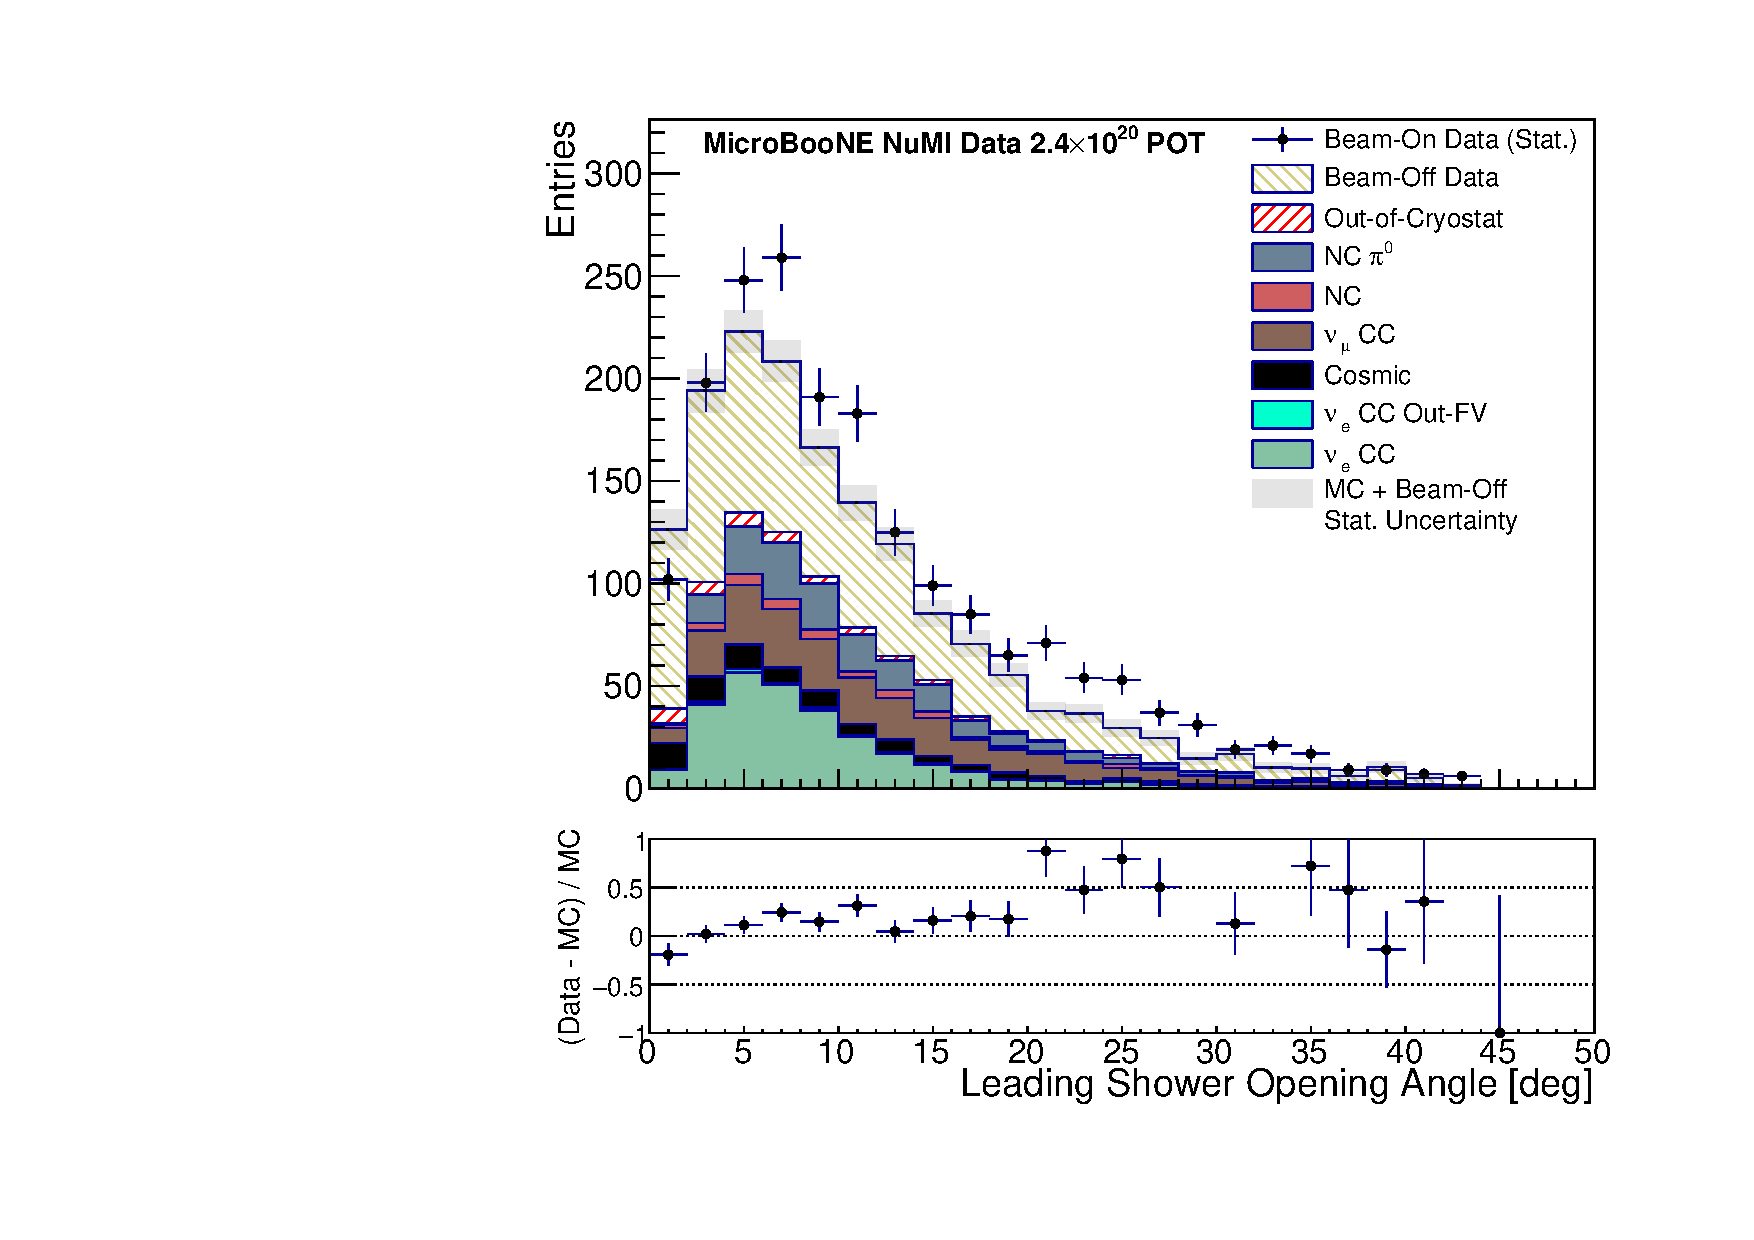
\includegraphics[width=0.6\textwidth]{plots/post_cuts_leading_shower_open_angle_data.pdf}
\caption{Comparison of data (points) to the stacked prediction (Monte Carlo + NuMI EXT) for the leading shower opening angle. TPC Objects pass the selection cut for leading showers between  3$^{\circ}$ and 15$^{\circ}$. This plot is shown after all selection cuts from groups \textbf{(1)}, \textbf{(2)}, \textbf{(3)}, and \textbf{(4)} have been applied.}
\label{post_cuts_leading_shower_open_angle_data}
\end{figure}

\FloatBarrier
%%%%%%%%%%%%%%%%%%%%%%%%%%%%%%%%%%%%%%%%%%%%%%%%%%%%%%%%%%
\subsubsection{Shower dE/dx}\label{section_dedx_cut}

One of the most powerful aspects of using a LArTPC is that whole volume is an active calorimeter. This means that the energy loss of a particle can be observed cleanly along its trajectory and it enables the use of the energy-loss per unit length (dE/dx) to perform particle ID. Examining the dE/dx in the first few centimetres of a shower can distinguish electron-induced from photon-induced showers, as was demonstrated by the ArgoNeuT detector \cite{argoneut}. In ArgoNeuT's studies they selected the median dE/dx value as a truer representation of the shower's deposition profile rather than the arithmetic mean. This mitigates effects from single outlier hits which could result from either misconfigured electronics, detector effects or mis-reconstruction.

The calculation of the median dE/dx is performed by constructing a $1$ $\times$ $4$ cm$^2$ box around the reconstructed shower start point (starting in the reconstructed shower direction) and examining the steps in charge deposition. Figure \ref{dedx_schematic} shows a very rough schematic of this technique.

\begin{figure}[htbp]
\center
\includegraphics[width=0.6\textwidth]{plots_main/dedx_schematic.pdf}
\caption{Rough schematic of the method used to calculate dQ/dx for reconstructed shower objects. The black lines represent a shower in the TPC. The blue box is the region used for calculating the dQ/dx and the red $x$ shows the reconstructed shower vertex. }\label{dedx_schematic}
\end{figure}

Figure \ref{post_cuts_dedx_cuts_data} shows the distribution of the calculated dE/dx on the collection plane wires for the leading shower using this method. The signal distribution peaks in the 2 MeV/cm region and large fractions of background lie to either side of the peak. By placing a cut between 1.4 MeV/cm and 3 MeV/cm the purity of the sample increases greatly. As expected, the TPC Objects containing photon-producing processes are centred around 4 MeV/cm. Overall agreement between data and prediction is good.

\begin{figure}[htbp]
\center
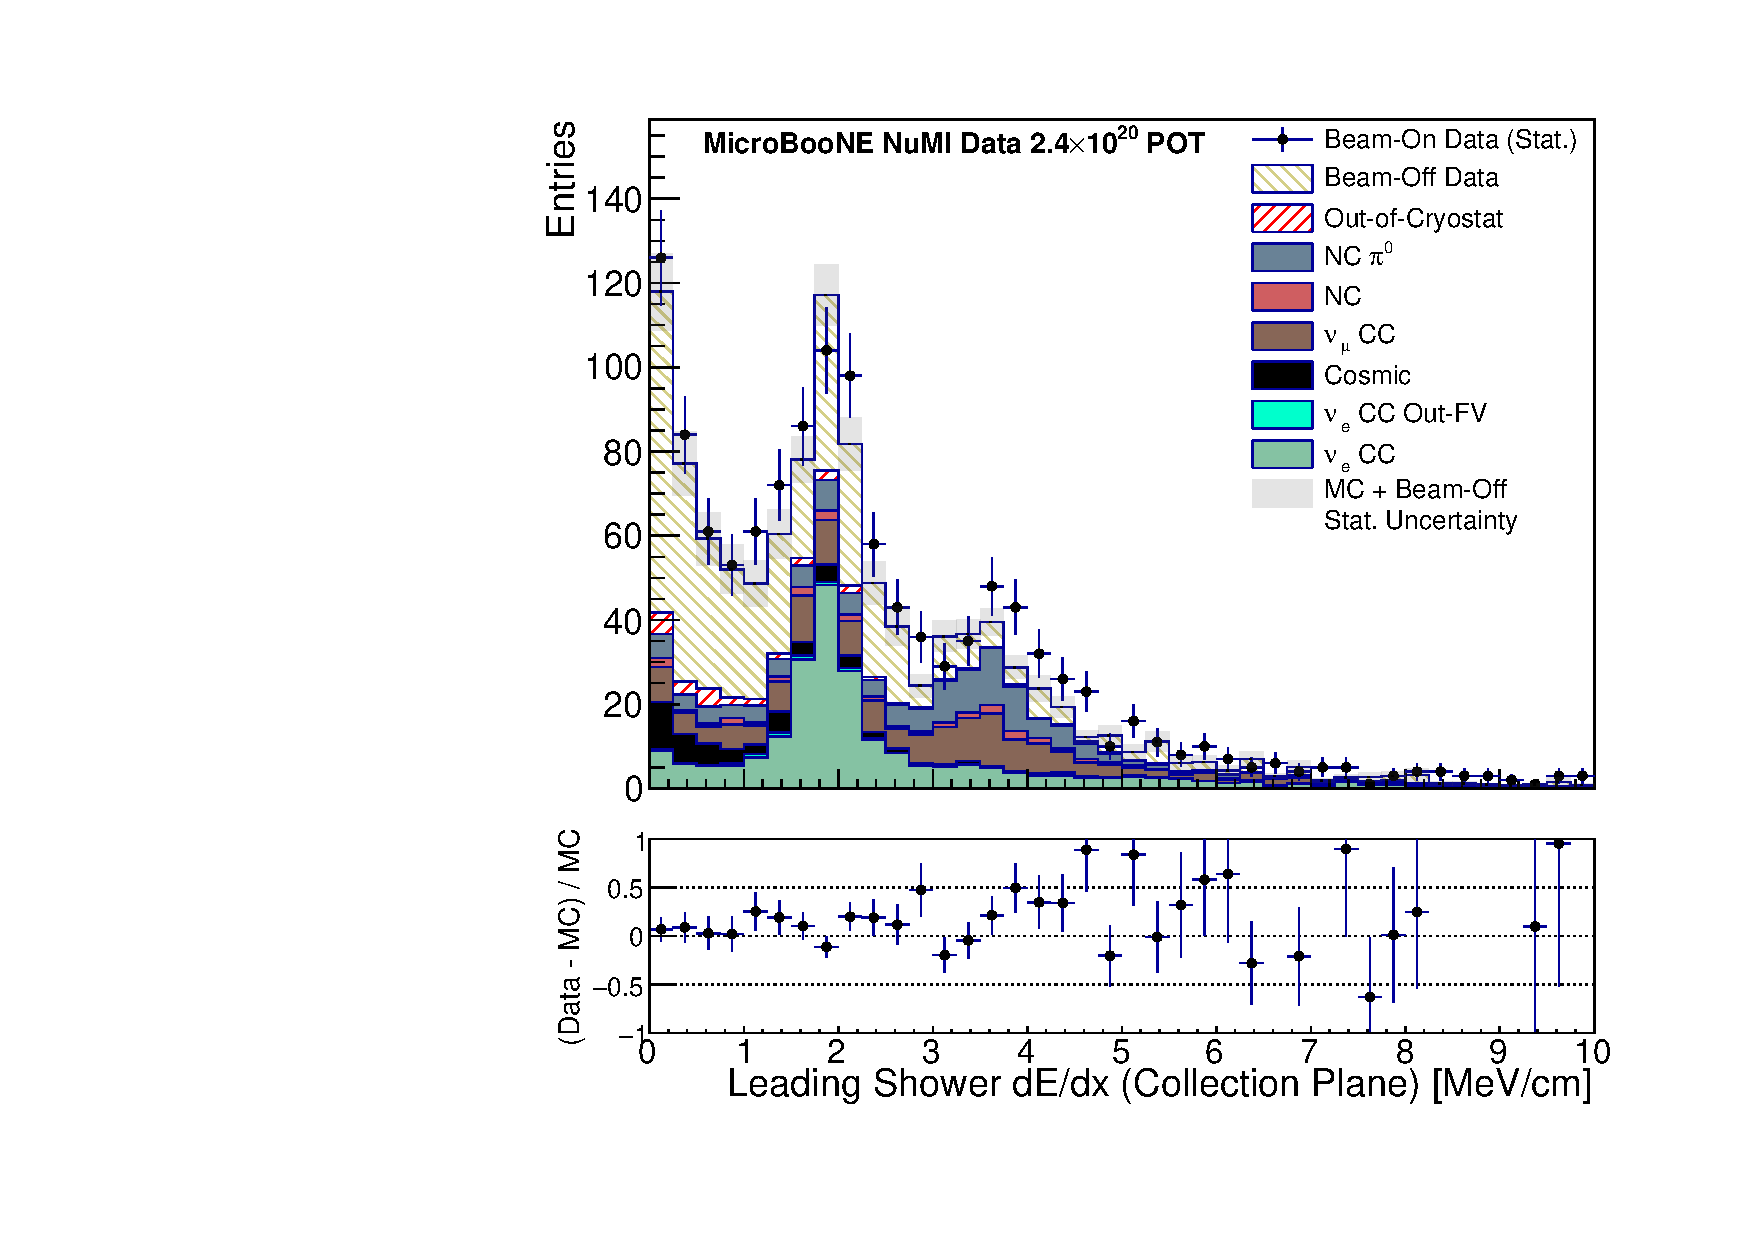
\includegraphics[width=0.6\textwidth]{plots/post_cuts_dedx_cuts_data.pdf}
\caption{Comparison of data (points) to the stacked prediction (Monte Carlo + NuMI EXT) for the leading shower dE/dx distribution following the opening angle selection cut. Signal interactions are peaked at 2 MeV/cm and beam-induced backgrounds are mostly peaked around 4 MeV/cm. Large amount of backgrounds are between 0 and 2 MeV/cm.}\label{post_cuts_dedx_cuts_data}
\end{figure}

A notable feature in Figure \ref{post_cuts_dedx_cuts_data} is the large population of signal leading showers with a dE/dx of nearly 0. This effect is caused by the ``dx'' value used in the calculation, which can become very large if the track or shower is parallel to the wires. This could be mitigated by using all three planes for the dE/dx calculation, however only the collection plane has shown reasonable data-Monte Carlo agreement to this point \cite{microboone_calibration_note}.

This unfortunately means that the shower dE/dx can heavily depend on the angle of the shower w.r.t the collection plane wires. Figure \ref{post_cuts_dEdx_theta_pre_cuts_data} demonstrates the relationship between the shower dE/dx and the angle of the shower w.r.t the collection plane wires. For angles between 0 - 60 and 120 - 180 degrees, the dE/dx does not have much angular dependence. However between about 70 and 110 degrees, the value of dE/dx is strongly influenced by the shower angle. In the future, the hope is to mitigate this issue by introducing the induction plane information. However without the simulation of induced charge effects and 2D deconvolution signal processing, using the induction planes would be unreliable, leading to a loss in efficiency \cite{microboone_calibration_note}.

\begin{figure}[htbp]
\center
\includegraphics[width=0.6\textwidth]{plots_main/post_cuts_dEdx_theta_pre_cuts_data.pdf}
\caption{Leading shower dE/dx vs leading shower $\theta$ for On-Beam data following the leading shower opening angle cut. For showers with dE/dx less than about 0.5 MeV/cm, the showers exclusively have reconstructed angles between 80 and 100 degrees. This aligns them parallel, or almost parallel, to the collection plane wires.}\label{post_cuts_dEdx_theta_pre_cuts_data}
\end{figure}

\begin{figure}[htbp]
\center
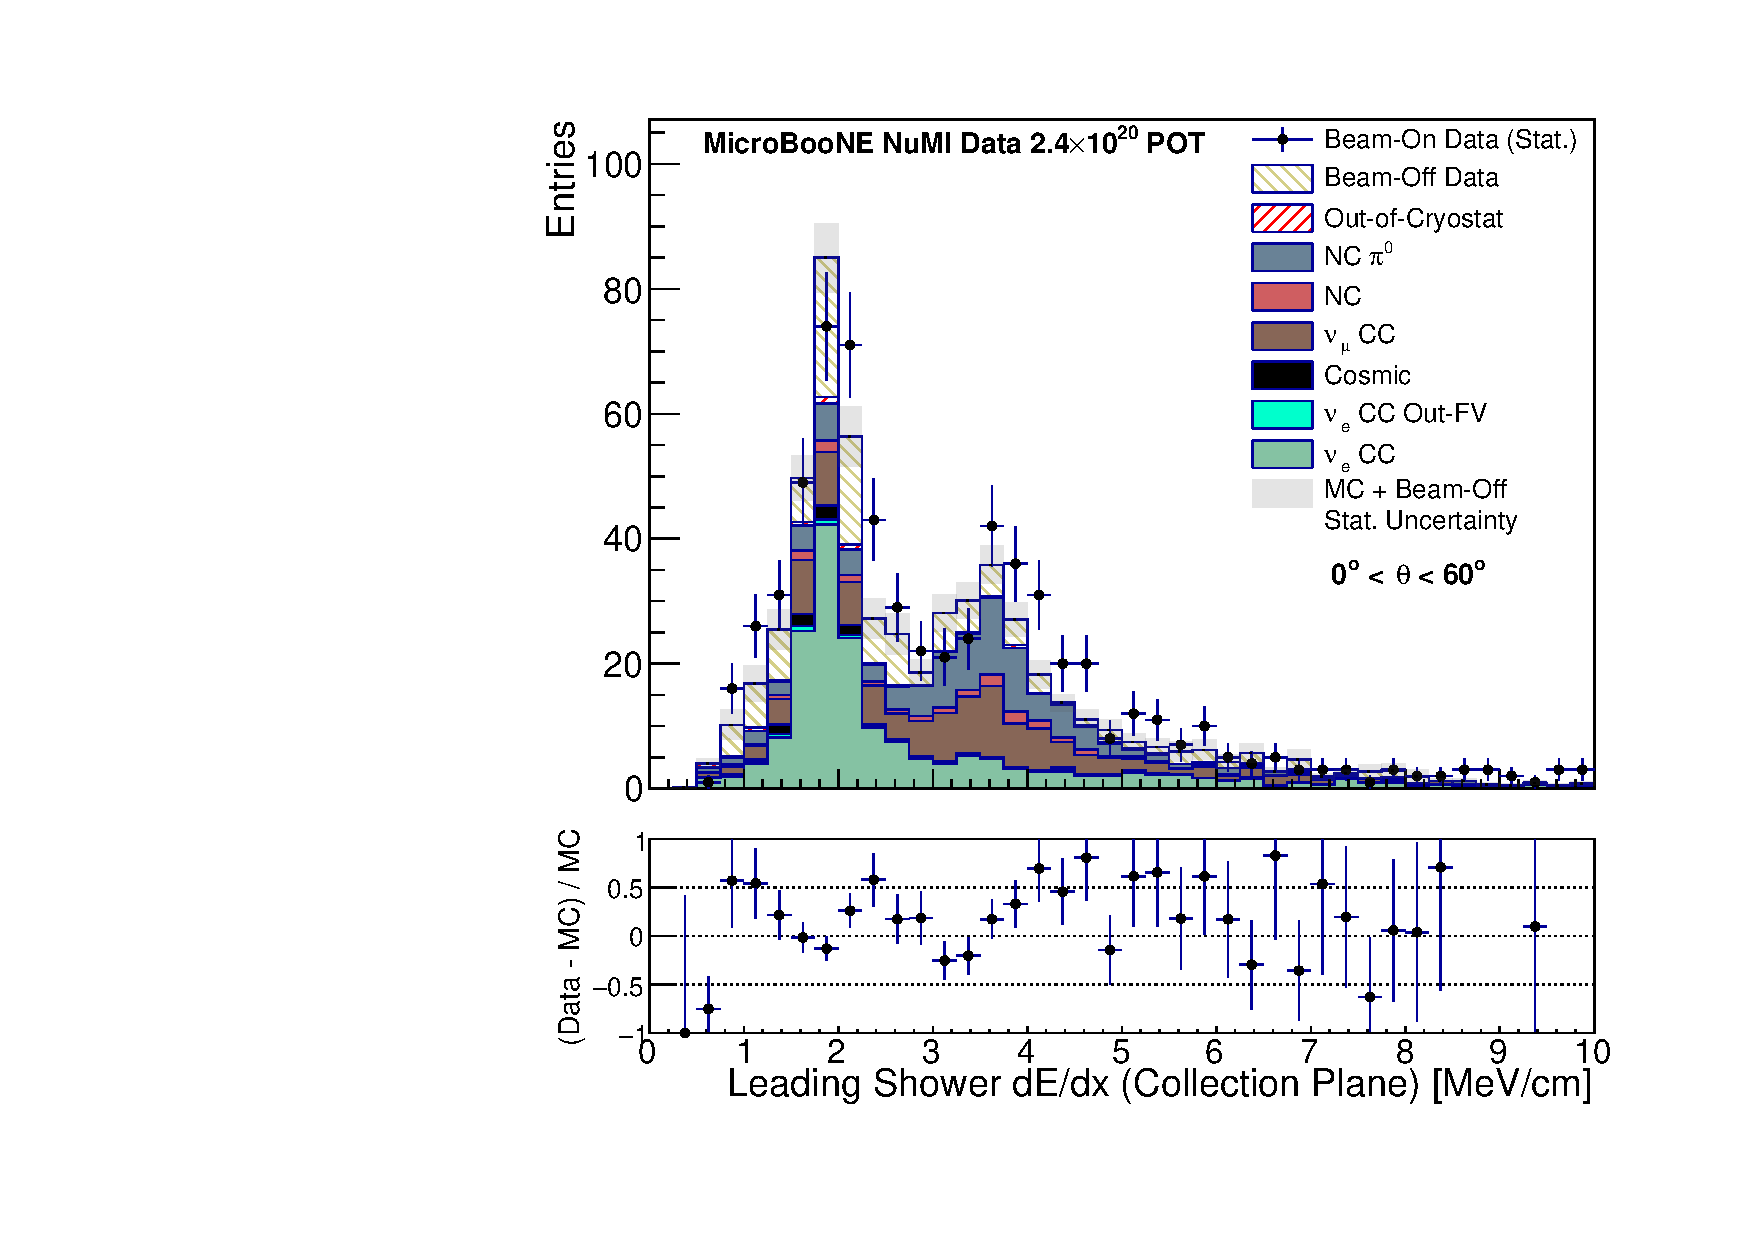
\includegraphics[width=0.48\textwidth]{plots/post_cuts_dedx_theta_slice_1_data.pdf}
\includegraphics[width=0.48\textwidth]{plots/post_cuts_dedx_theta_slice_1_zoom_data.pdf}
\caption{Comparison of data (points) to the stacked prediction (Monte Carlo + NuMI EXT) for the leading shower dE/dx for a slice of $\theta$ between 0 and 60 degrees after the shower opening angle cut. The signal peak is well-defined and few leading showers have a poorly reconstructed dE/dx. Plot on the right is an X-axis zoom into the signal region (0 to 4 MeV/cm).}
\label{post_cuts_dedx_theta_slice_1_data}
\end{figure}

\begin{figure}[htbp]
\center
\includegraphics[width=0.48\textwidth]{plots/post_cuts_dedx_theta_slice_2_data.pdf}
\includegraphics[width=0.48\textwidth]{plots/post_cuts_dedx_theta_slice_2_zoom_data.pdf}
\caption{Comparison of data (points) to the stacked prediction (Monte Carlo + NuMI EXT) for the dE/dx of the leading shower, for a slice of $\theta$ between 60 and 120 degrees after the shower opening angle cut. Some leading showers are still well-reconstructed, however a number of showers have almost 0 MeV/cm. Cosmic contamination in this slice is much higher than in the 0 to 60 degree region. Plot on the right is an X-axis zoom into the signal region (0 to 4 MeV/cm).}
\label{post_cuts_dedx_theta_slice_2_data}
\end{figure}

\begin{figure}[htbp]
\center
\includegraphics[width=0.48\textwidth]{plots/post_cuts_dedx_theta_slice_3_data.pdf}
%\includegraphics[width=0.6\textwidth]{plots/post_cuts_dedx_theta_slice_3_zoom_data.pdf}
\caption{Comparison of data (points) to the stacked prediction (Monte Carlo + NuMI EXT) for the dE/dx of the leading shower, for a slice of $\theta$ between 120 and 180 degrees after the shower opening angle cut. Most leading showers have a well-reconstructed dE/dx. Statistics in this $\theta$ slice are low.}
\label{post_cuts_dedx_theta_slice_3_data}
\end{figure}

To further illustrate the angular dependence of the dE/dx calculation, Figures \ref{post_cuts_dedx_theta_slice_1_data}, \ref{post_cuts_dedx_theta_slice_2_data} and \ref{post_cuts_dedx_theta_slice_3_data} show the stacked data versus prediction for three different slices of $\theta$. Figure \ref{post_cuts_dedx_theta_slice_1_data} shows the most populated and well-defined region, where $\theta$ is between 0 and 60 degrees. This slice of $\theta$ also has considerably higher purity than other slices of $\theta$. As the dE/dx does not suffer from showers running parallel to the wires in this angular slice, a very small fraction of showers have an unphysically low dE/dx.

Figure \ref{post_cuts_dedx_theta_slice_2_data} shows the leading shower dE/dx for a slice of $\theta$ from 60 to 120 degrees. The cosmic contamination is considerably higher for this slice, and the TPC Objects are peaked near 0 MeV/cm. This is the region of shower direction where the dE/dx is expected to be worst-defined. The behaviour seems to be modelled well by the Monte Carlo.

The last slice goes from 120 to 180 degrees. This region of reconstructed shower phase-space has relatively few entries, and as seen in Figure \ref{post_cuts_dedx_theta_slice_3_data}, is background dominated. Some signal interactions are located near the MIP peak and the majority of leading showers seem to have a well-defined dE/dx. The cosmic contamination in this region is relatively high.

\begin{figure}[htbp]
\center
\includegraphics[width=0.6\textwidth]{plots_main/post_cuts_dedx_true_particle.pdf}
\caption{dE/dx of leading showers for TPC Objects which have passed all cuts including the leading shower opening angle cut. Instead of the TPC Object category, the true particle type is shown. Electrons are gathered in the MIP peak, while most photons are around 4 MeV/cm.}
\label{post_cuts_dedx_true_particle}
\end{figure}

Given that the reconstructed leading shower direction can affect the calculation of the dE/dx, the direction becomes a very relevant factor for the event selection. Potentially, application of a dE/dx cut introduces a bias to the selection. To avoid this, it was considered to only remove leading showers with values of dE/dx above 3 MeV/cm. By not cutting around 0 MeV/cm, this would potentially remove the bias in $\theta$ between 60$^{\circ}$ and 120$^{\circ}$. However, much of the power of the dE/dx cut comes from removing non-MIP-like cosmic and beam-induced backgrounds, which are also found at low values of dE/dx. Relaxing the cut causes a significant drop in the selection performance, concluding that the loss in $\theta$ sensitivity around 90 degrees is necessary.

The dE/dx selection cut also effectively removes photon-induced backgrounds. Figure \ref{post_cuts_dedx_true_particle} shows the dE/dx classified by the true particle types, with event rates scaled to the On-Beam~POT. For the peak around 2 MeV/cm, mostly electron showers are present, consistent with the selection cut for signal interactions. Around 4 MeV/cm photons dominate. This confirms that the behaviour of reconstructed showers in Monte Carlo is well modelled and that cutting to isolate the MIP peak should reduce primarily background particles. A supplementary study looking in detail at TPC Objects in the photon peak can be found in Appendix \ref{photon_background_section}.

\FloatBarrier
%%%%%%%%%%%%%%%%%%%%%%%%%
\subsubsection{Shower Like-ness Summary}

This set of cuts is impactful in removing not only photon-induced shower backgrounds, but also cosmic and $\nu_{\mu}$ CC interactions. For regions where the dE/dx is well defined, the effectiveness of the cut is clear - efficiency drops by 13\% to a total of 13.21\%, but purity increases by about 16\% to a total of 29.28\%. Table \ref{selection_summary_table_dedx} shows the selection performance breakdown following these shower like-ness cuts.

\begin{table}[htbp]
\center
\begin{tabular}{l | l l }
Classification & Num. Remaining & Rel. Remaining [\%] \\
\hline
$\nu_e$ CC & 122.03 & 50.56\\
$\nu_e$ CC Mixed & 17.56 & 48.9\\
$\nu_e$ CC OutFV & 3.38 & 35.58\\
$\nu_{\mu}$ CC & 51.78 & 21.17\\
NC & 4.03 & 18.66\\
NC $\pi^0$ & 33.96 & 20.27\\
NC Mixed & 4.55 & 23.16\\
Unmatched & 0.13 & 7.14\\
Cosmic & 15.61 & 18.90\\
InTime & 156.37 & 21.57\\
Dirt & 7.55 & 16.91\\
\hline
\hline
Efficiency & 13.21\%\\
Purity & 29.28\%\\
\hline
On-Beam Data & 453\\
\hline
\end{tabular}
\caption{Breakdown of remaining TPC Objects by classification type following the dE/dx cut, normalised to the On-Beam POT. The relative percentages are compared to the values following selection cuts \textbf{(1)}, \textbf{(2)}, \textbf{(3)} and \textbf{(4)}. }\label{selection_summary_table_dedx}
\end{table}

\FloatBarrier
%%%%%%%%%%%%%%%%%%%%%%%%%%%%%%%%%%%%%%%%%%%%%%%%%%%%%%
%%%%%%%%%%%%%%%%%%%%%%%%%%%%%%%%%%%%%%%%%%%%%%%%%%%%%%
\subsection{Final Tuning Cuts}

\subsubsection{Secondary Shower Distance}

In some cases, TPC Objects can be mis-reconstructed with physically uncorrelated showers associated to TPC Objects. A similar cut to those used in \textbf{(3)} is constructed, comparing the distance between the secondary showers and the TPC Object vertex. To prevent unintentionally removing signal $\pi^0$ TPC Objects, the cut threshold is placed at more than 22 cm from the reconstructed neutrino vertex, where the characteristic conversion distance is 11 cm in argon. Figure \ref{post_second_shwr_dist_data} includes only TPC Objects with 2 or more showers and plots the secondary shower properties only. Most TPC Objects fall off quickly at distances greater than about 10 cm, and the large fraction of TPC Objects removed are ``mixed''. This cut does on average remove more resonant signal interactions compared to QE/MEC signal interactions (See Table \ref{interaction_breakdown_table}), but results in a minor increase in purity.

\begin{table}[htbp]
\center
\begin{tabular}{l | l | l | l}
Type & Before & After & \% Remaining\\
\hline
QE & 61.28 & 53.47 & 87.26\\ 
Res & 30.18 & 22.51 & 74.58\\
DIS & 8.20 & 4.94 & 60.32\\
Coh & 0.52 & 0.39 & 75.0\\
MEC & 21.86 & 19.25 & 88.10\\
\hline
\end{tabular}
\caption{Breakdown of signal TPC Objects based on interaction mode after cut group \textbf{(5)}. Values are shown for immediately before and immediately after the selection cut on the reconstructed secondary shower vertex. A larger fraction of resonant and DIS interactions are removed than QE and MEC interactions.}\label{interaction_breakdown_table}
\end{table}

\begin{figure}[htbp]
\center
\includegraphics[width=0.48\textwidth]{plots/post_second_shwr_dist_data.pdf}
\includegraphics[width=0.48\textwidth]{plots_main/post_second_shwr_dist_data_logy.pdf}
\caption{Comparison of data (points) to the stacked prediction (Monte Carlo + NuMI EXT) for the distance between the reconstructed TPC Object vertex and all shower vertices beyond the leading shower, following selection cut group \textbf{(5)}. The tail of the distribution continues beyond 80 cm. The figure to the right is plotted with a Log(Y)-axis.}\label{post_second_shwr_dist_data}
\end{figure}

%%%%%%%%%%%%%%%%%%%%%%%%%%%%%%%%%%%%%%%%%%%%%%%%%%%%%%%%%%
\subsubsection{Hit Per Length Ratio}

The contamination from primarily cosmic rays is still relatively dominant following the selection cuts used so far. This selection cut is constructed by summing the number of hits associated to the leading shower and dividing by its length. Figure \ref{post_hit_length_ratio_data} illustrates how backgrounds largely populate lower values of hits per length of the leading shower. While some separation power is evident, to get substantial gains, large amounts of signal would need to be sacrificed. Therefore, the threshold is conservatively placed at 3 hits per cm. Note, effectiveness of this selection cut is particularly sensitive to reconstruction of the transverse component of the shower. 

\begin{figure}[htbp]
\center
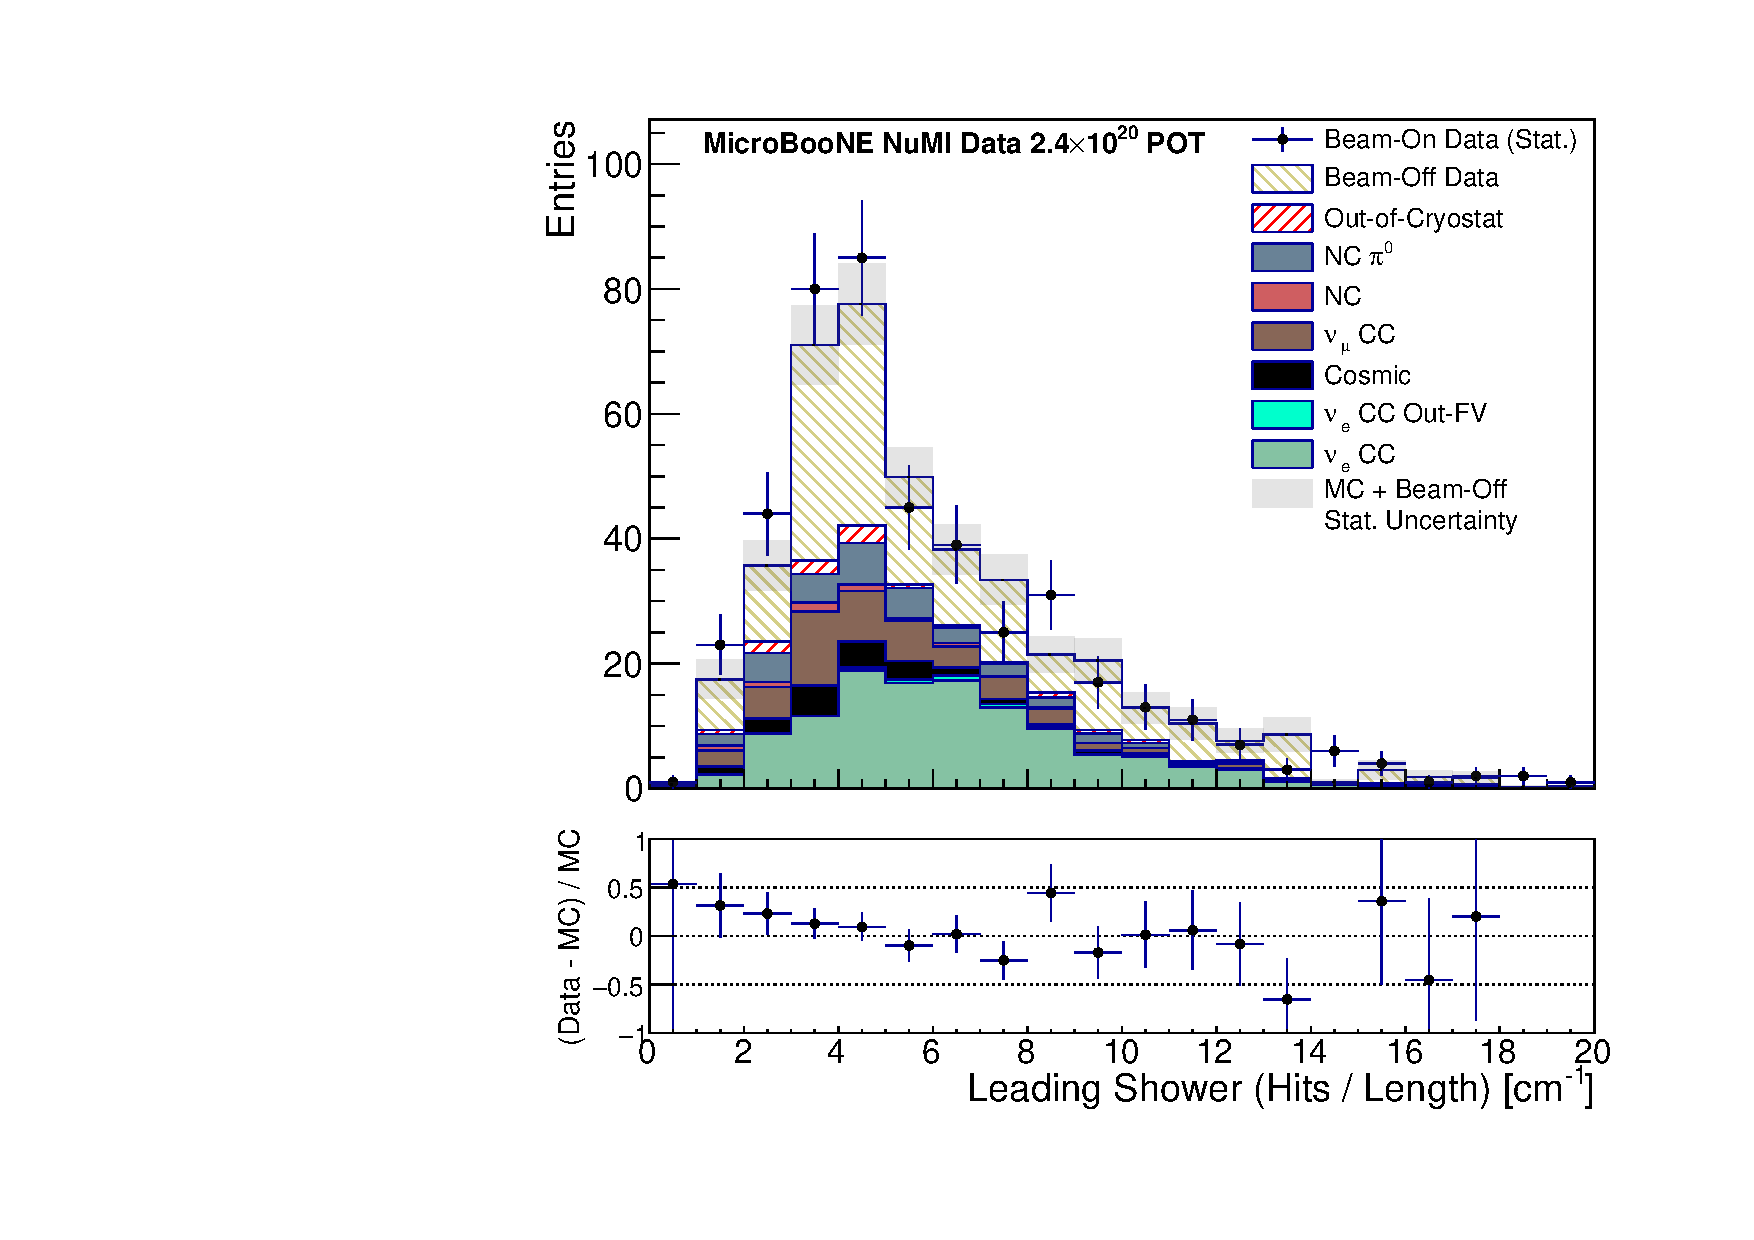
\includegraphics[width=0.6\textwidth]{plots/post_hit_length_ratio_data.pdf}
\caption{Comparison of data (points) to the stacked prediction (Monte Carlo + NuMI EXT) for the number of hits per length for the leading shower after the secondary shower distance cut. Background TPC Objects are peaked at lower values. Cutting conservatively, the threshold is placed at 3 hits per cm. If efficiency is less of a concern, there is potential to achieve higher purity by increasing the threshold to 5 or 6 hits per cm.}\label{post_hit_length_ratio_data}
\end{figure}

Reconstructed showers failing this cut are expected to either be true track objects or poorly reconstructed true shower objects. This selection cut has a few percent effect on the overall selection purity and efficiency. A higher purity, but lower efficiency sample could be obtained by increasing the hits per cm to 5, increasing the purity roughly 10\% further, while efficiency falls an additional 2\%. This would impact low energy signal efficiency the most, where reconstruction has more difficulty identifying showers in their entirety. As such, the threshold is maintained at 3 cm$^{-1}$ for this analysis, but could be increased in future iterations.

%%%%%%%%%%%%%%%%%%%%%%%%%%%%%%%%%%%%%%%%%%%%%%%%%%%%%%%%%%
\subsubsection{Track to Shower Ratio}

A relationship between track and shower objects produced by well-reconstructed interactions is expected, namely the ratio between the length of the longest track and leading shower. For example a $\nu_{\mu}$ CC interaction would have a rather long $\mu$, and any showers associated to the interaction would be much shorter in length. Whereas for a $\nu_e$ CC interaction, the tracks produced should be of comparable length or less than the shower length, even in the presence of charged pions. Such a cut can also remove cases where Michel electrons are produced by $\nu_{\mu}$ or mixed interactions. The cut parameter shown in Figure \ref{post_leading_shower_trk_lengths_data} is defined as the longest track in the TPC Object divided by the leading shower lengths with the cut value placed at 1.0. 

\begin{figure}[htbp]
\center
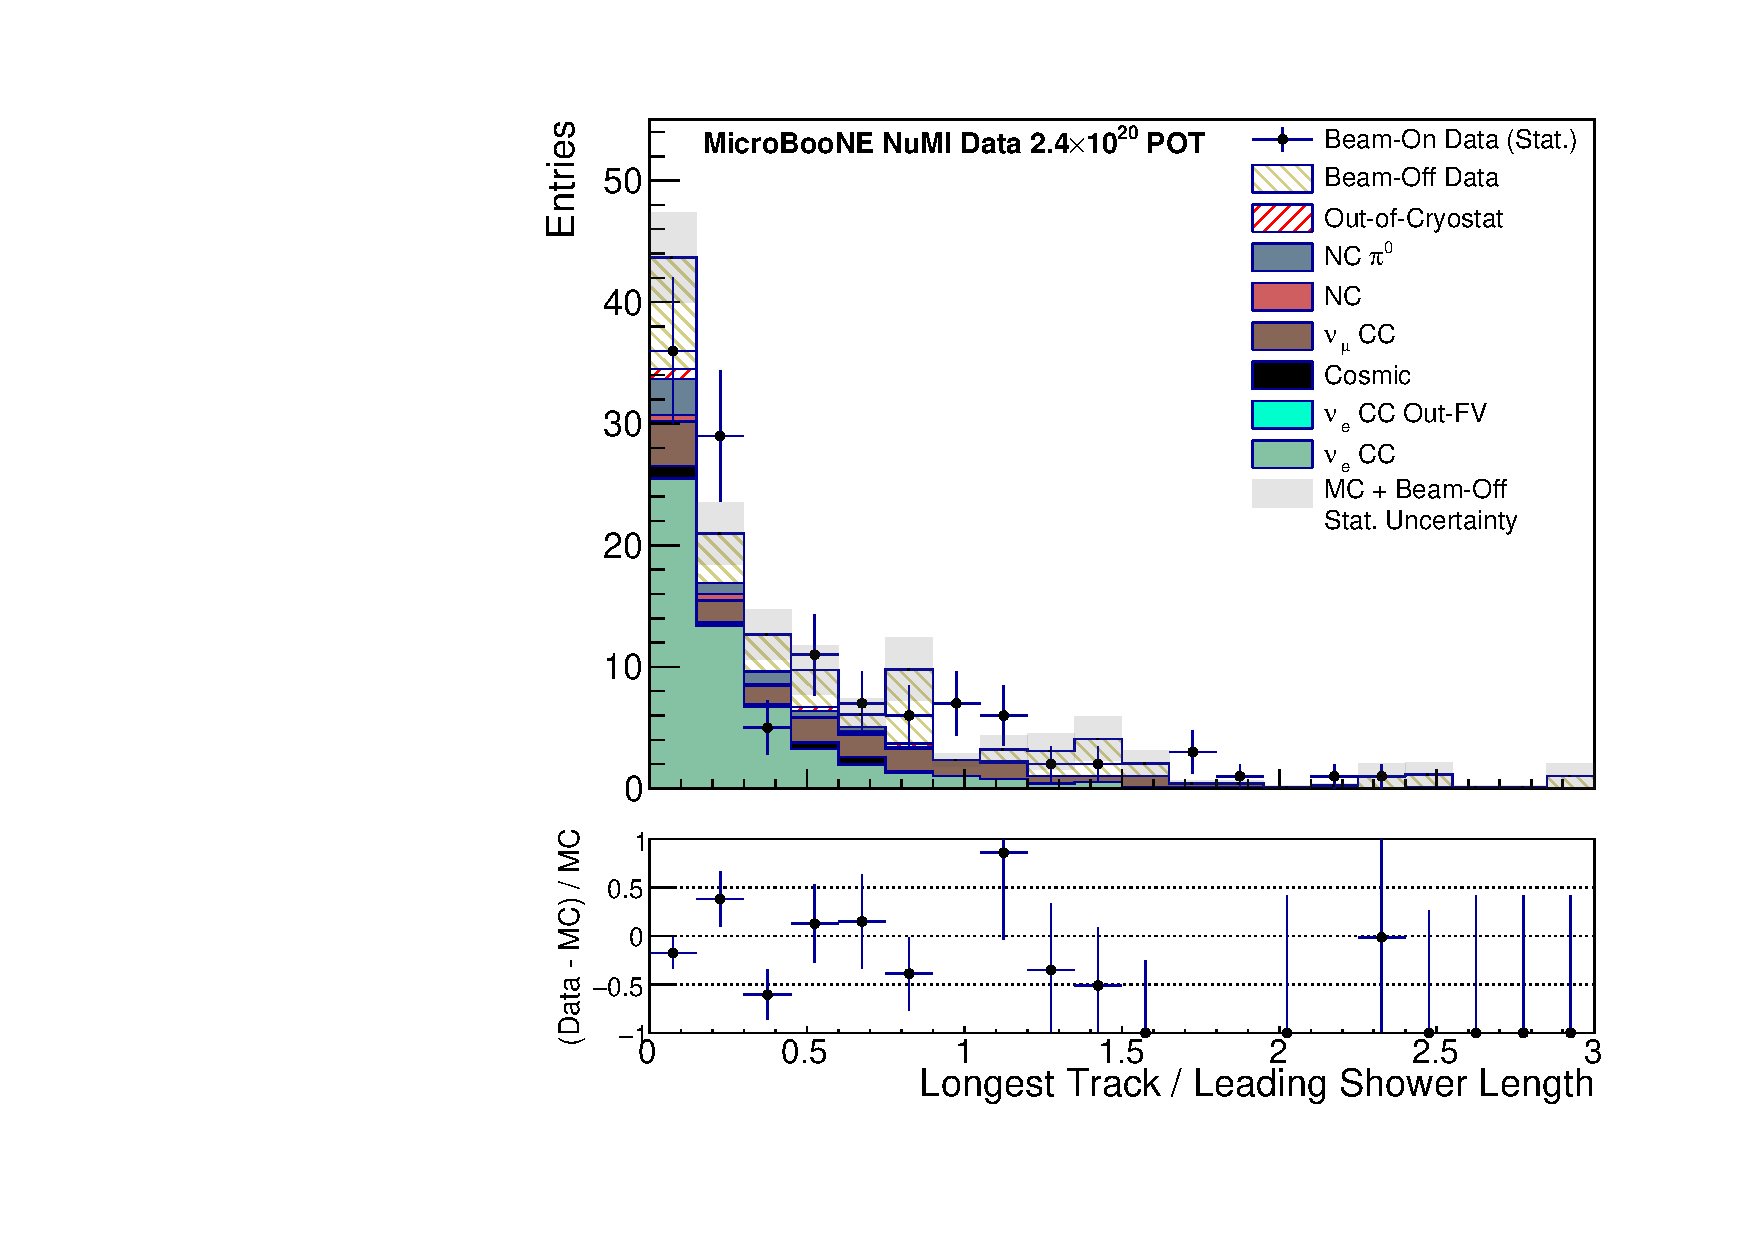
\includegraphics[width=0.6\textwidth]{plots/post_leading_shower_trk_lengths_data.pdf}
\caption{Comparison of data (points) to the stacked prediction (Monte Carlo + NuMI EXT) for the ratio between the longest track and the leading shower lengths following the cut on the shower hits per length. The threshold is placed at 1.0, where all TPC Objects that have a track longer than the leading shower are removed.}\label{post_leading_shower_trk_lengths_data}
\end{figure}

%%return%% -- 2D distribution of longest track length vs leading shower length for signal and background events

\FloatBarrier
%%%%%%%%%%%%%%%%%%%%%%%%%%%%%%%%%%%%%%%%%%%%%%%%%%%%%%%%%%
\subsubsection{Track Containment}

The final selection cut takes another pass at increasing the purity of shower + track topologies, by requiring that both the reconstructed start and end of the track are contained inside the fiducial volume. This is particularly useful for long cosmic rays or muons which cross the fiducial volume and are associated to a shower inside the fiducial volume. Figure \ref{track_containment} shows the fraction of TPC Objects which pass or fail the track containment requirement. This has a very small impact on signal interactions, and results in a roughly 3\% increase in the purity. As a note: this cut only applies to TPC Objects with 1 or more tracks. The purity inferred from Figure \ref{track_containment} is for TPC Objects with tracks and is not the final inclusive selection purity. 

\begin{figure}[htbp]
\center
\includegraphics[width=0.6\textwidth]{plots/track_containment_data.pdf}
\caption{Comparison of data (points) to the stacked prediction (Monte Carlo + NuMI EXT) for the distribution of TPC Objects which have all tracks contained (1) and any uncontained tracks (0) following the track to shower ratio cut. The number of signal TPC Objects compared to background interactions being removed is relatively low. There are relatively few entries in this plot, as this only includes TPC Objects with at least one track.}\label{track_containment}
\end{figure}


\subsubsection{Final Tuning Cuts Summary}

The number of final remaining TPC Objects after these and all previous selection cuts are shown in Table \ref{selection_summary_track_containment}. Primarily cosmic and $\nu_{\mu}$ CC backgrounds were removed by the finalisation cuts in addition to a handful of NC interactions. Overall, this group of cuts resulted in about a 4\% drop in efficiency and an increase of about 10\% in purity.

\begin{table}[htbp]
\center
\begin{tabular}{l | l l }
Classification & Num. Remaining & Rel. Remaining [\%]\\
\hline
$\nu_e$ CC & 85.52 & 70.08\\
$\nu_e$ CC Mixed & 0.26 & 1.48\\
$\nu_e$ CC OutFV & 1.82 & 5.38\\
$\nu_{\mu}$ CC & 14.31 & 27.64\\
NC & 2.08 & 51.61\\
NC $\pi^0$ & 17.17 & 50.56\\
NC Mixed & 0.39 & 8.57\\
Unmatched & 0.13 & - \\
Cosmic & 10.15 & 65.02\\
InTime & 82.25 & 52.60\\
Dirt & 4.92 & 65.17\\
\hline
\hline
Efficiency & 9.03\%\\
Purity & 38.49\%\\
\hline
On-Beam Data & 214\\
\hline
\end{tabular}
\caption{Breakdown of remaining TPC Objects by classification type following the track containment cut, normalised to the On-Beam POT. Values shown here enter into the cross section calculation, as this is the final selection cut. The relative values are following all cuts before the finalisation cut group.}
\label{selection_summary_track_containment}
\end{table}

\FloatBarrier
%%%%
\subsection{Selection Performance}

Many of the selection cuts focus on removing cosmic ray interactions which have been reconstructed as a shower. The overall decrease in the cosmic ray contamination is a factor $\approx$100,000 from the initial selection cuts and ultimately brings the cosmic ray contamination to roughly the same size as the selected true signal events. With the cosmic ray tagger (CRT) system installed around MicroBooNE and available for future selections, contamination from cosmic ray backgrounds should severely decrease. Significant gains in performance, especially in purity are expected. The remaining non-cosmic backgrounds contribute only $\approx$15\% to the selected TPC Objects. This demonstrates the selection's ability to reliably remove beam-induced backgrounds such as $\nu_{\mu}$ CC and $\pi^{0}$ interactions. 

A summary of the purity and efficiency as a function of the selection cuts can be seen in Figure \ref{efficiency_purity}. This figure includes the efficiency (green), purity (blue) and the beam-only purity (purple). %On the X-axis are the cut label names, where they correspond to the values following the application of the listed cut. Not every selection cut is displayed in the plot, and as such their effects are combined in the figure.

The efficiency continually declines as selection cuts are applied. The steepest decrease occurs with the applications of the shower opening angle and dE/dx cuts (group \textbf{(5)}~), specifically where signal TPC Objects were removed because of the difficulty in calculating dE/dx for certain shower directions. Examining the purity at this same point, this is also where the purity rises the most. With improvements to calculating dE/dx for all shower directions, this cut is expected to become even more powerful, by reducing the efficiency loss and increasing purity gains.

Finally, the beam-only purity is calculated by considering only beam-induced backgrounds. In the case that all cosmic ray backgrounds can be perfectly removed from the selected TPC Objects (e.g. by adding information from the CRT), this iteration of the selection would achieve a purity above 60\%. This suggests that the beam-induced backgrounds are relatively well constrained and investing time into further cosmic rejection would produce considerable benefits.

\begin{figure}[htbp]
\center
\includegraphics[width=0.95\textwidth]{python/plots/efficiency_purity_beam_only_grid.pdf}
\caption{Summary of the selection performance, including efficiency, purity, and purity (beam only). The beam only purity corresponds to the selection purity if cosmic rejection is perfect, and gives a projection of the selection performance when the CRT is employed. Note that the efficiency does not start at 100\%, as over 30\% of the true $\nu_e$/$\bar{\nu}_e$ events are not reconstructed.}\label{efficiency_purity}
\end{figure}
